\documentclass[12pt]{article}
 
\usepackage[margin=.5in]{geometry} 
\usepackage{amsmath,amsthm,amssymb,outlines}
\usepackage{graphicx,tikzsymbols,tcolorbox}
\renewcommand\qedsymbol{$\blacksquare$}
\tcbuselibrary{most}

\newtcolorbox{newtitle}{
  enhanced,
  colframe=black,
  colback=white,
  boxsep=5pt,
  arc=8pt,
  sharp corners=south,
  borderline={0.5pt}{0pt}{black},
  borderline={1.8pt}{-5pt}{black},
  after skip=30pt
}

\newtcolorbox[auto counter]{statement}[1][]{
  enhanced,
  title={Exercise \ifx\\#1\\\thetcbcounter\else#1\fi},
  colframe=black,
  colback=white,
  colbacktitle=white,
  fonttitle=\bfseries,
  coltitle=black,
  attach boxed title to top left={yshift=-0.25mm-\tcboxedtitleheight/2,yshifttext=2mm-\tcboxedtitleheight/2, xshift=2mm},
  boxed title style={boxrule=0.5mm}
}

\newtcolorbox{newproof}{
  enhanced,
  breakable,
  frame hidden,
  colback=white,
  title={Proof.},
  fonttitle=\bfseries,
  coltitle=black,
  colbacktitle=white,
  boxed title style={boxrule=0.5mm},
  attach boxed title to top left={yshift=-0.25mm-\tcboxedtitleheight/2,yshifttext=2mm-\tcboxedtitleheight/2, xshift=2mm},
  borderline west={1.5pt}{8pt}{black},
  after upper={\hfill $\blacksquare$}
}

\begin{document}

\begin{newtitle}
  \begin{center}
    \textbf{\Huge 8150 Homework III}
  \end{center}
  \textbf{Dahlen Elstran} \hfill \textbf{\today}
\end{newtitle}

\section*{Stein Problems}

% Problem 1

\begin{statement}[1]
  Using Euler's Formula
  $$ \sin \pi z = \frac{e^{i \pi z}-e^{-i \pi z}}{2i}, $$
  show that the complex zeroes of $\sin \pi z$ are exactly the integers, and that they are each of order 1. 
  \par Calculate the residue of $1/\sin \pi z$ at $z=n \in \mathbb{Z}$. 
\end{statement}
\begin{newproof}
  To find the zeroes, set Euler's Formula to zero:
  $$ \frac{e^{i \pi z}-e^{-i \pi z}}{2i} = 0. $$
  From here, we can find that 
  \begin{align*}
    e^{i \pi z} - e^{-i \pi z} &= 0 \\
    e^{i \pi z} &= e^{-i \pi z} \\ 
    i \pi z &= -i \pi z + 2 \pi i k , k \in \mathbb{Z} \\
    2i \pi z &= 2 i \pi k,
  \end{align*}
  so that $z = k$, meaning $z$ must be an integer. 
  \par To show that they are all of order one, we can find the derivate of $\sin \pi z$ to be 
  $ \pi \cos \pi z$, and notice that this is nonzero for any integer. 
  \par To find the residue of $1 / \sin \pi z$ at $z$ an integer, we can use this formula:
  $$ \text{Res}(f,a)=\lim_{z \to a} (z-a)(f(z)). $$
  So in our case, 
  $$ \text{Res}(\frac{1}{\sin \pi z}, n) = \lim_{z \to n} (z-n) \cdot \frac{1}{\sin \pi z}, $$
  where $n \in \mathbb{Z}$. 
  We know that near $z=n$, $\sin \pi z$ can be approximated using a Taylor Expansion, so that 
  $$ \frac{1}{\sin \pi z} \approx \frac{1}{\pi (z-n)(-1)^n}. $$
  Therefore we find that 
  $$ \text{Res}(\frac{1}{\sin \pi z}, n ) = \frac{1}{\pi (-1)^n}. $$
\end{newproof}

% Problem 2

\begin{statement}[2]
  Evaluate the inegral 
  $$ \int^{\infty}_{-\infty} \frac{dx}{1+x^4}. $$
  Where are the poles of $1/(1+z^4)$?
\end{statement}
\begin{newproof}
  First, to find the poles, we must find where $1+z^4=0$. This is at the points $z_0=e^{i \pi/4}, 
  z_1=e^{i 3 \pi/4}, z_2=e^{i 5 \pi/4}, z_3=e^{i 7 \pi/4}$. Then, we can contour over a semicircle 
  centered at the origin with radius $R$:
  \par \begin{center} 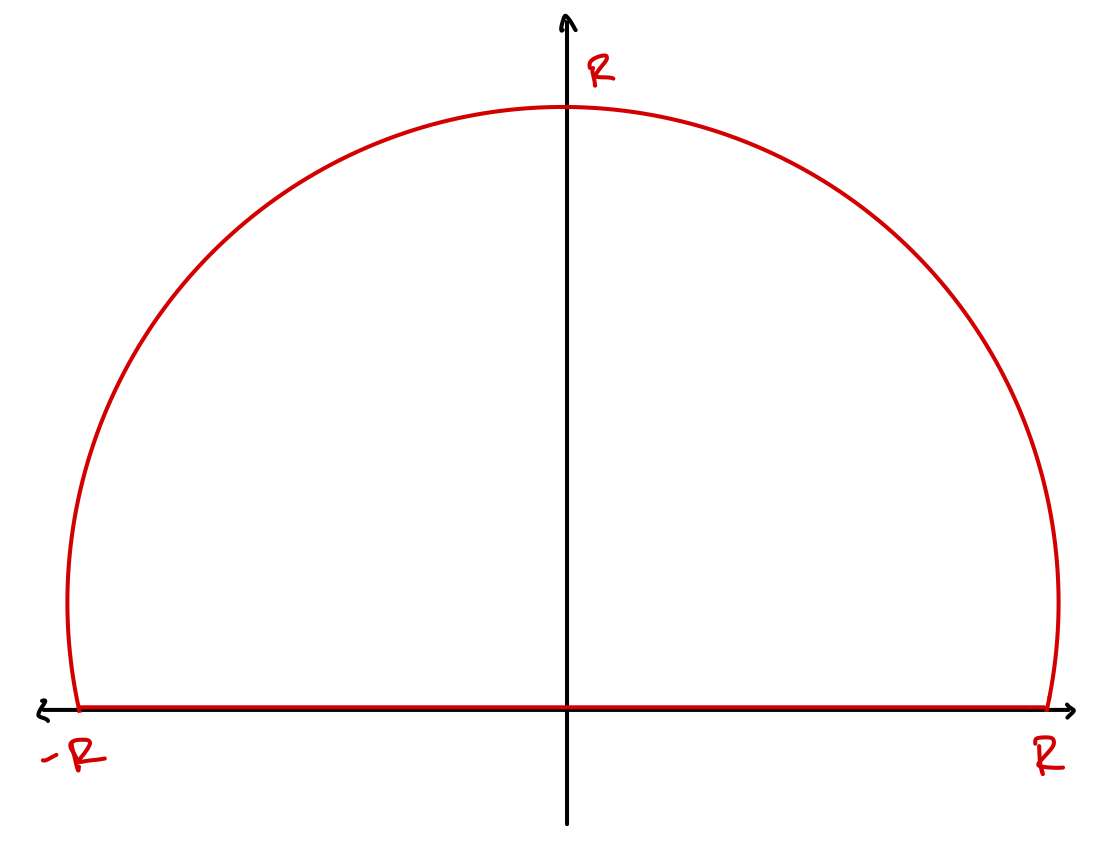
\includegraphics[scale=.2]{1.2-1.png} \end{center} 
  \par As $R \to \infty$, the integral vanishes because $\frac{1}{1+z^4}$ decays like $\frac{1}{\vert z \vert^4}$
  for large enough $\vert z \vert$. We're only concerned with the poles in the upper half of the plane, 
  so by the residue theorem, 
  $$ \oint \frac{dz}{1_z^4} = 2 \pi i (\text{Res}(z_0) + \text{Res}(z_1)). $$
  Calculating the residues, we find:
  $$ \text{Res}(z_0)= \lim_{z \to z_0} \frac{z-z_0}{1+z^4} = \frac{1}{4z_0^3} = \frac{1}{4} e^{-i 3 \pi /4} $$
  \begin{center} and, similarly, \end{center}
  $$ \text{Res}(z_1) = \frac{1}{4z_1^3}=\frac{1}{4}e^{-i9 \pi /4} = \frac{1}{4}e^{-i \pi /4}. $$
  \par Therefore we find that
  \begin{align*}
    \int^{\infty}_{-\infty} \frac{dx}{1+x^4} &= 2\pi i \left(\frac{1}{4}\left(e^{-i 3 \pi /4} + e^{-i \pi / 4}\right)\right) \\
                                             &= 2 \pi i \left( \frac{1}{4}\left(-\frac{\sqrt{2}}{2}-
                                             i\frac{\sqrt{2}}{2}+\frac{\sqrt{2}}{2}-i\frac{\sqrt{2}}{2}\right)\right) \\
                                             &= 2\pi i \left(-\frac{i\sqrt{2}}{4}\right) \\
                                             &= \frac{\pi \sqrt{2}}{2}.
  \end{align*}
\end{newproof}

% Problem 4

\begin{statement}[4]
  Show that 
  $$ \int^{\infty}_{-\infty} \frac{x \sin x}{x^2 + a^2} dx = \pi e^{-a}, \text{ for all } a > 0. $$
\end{statement}
\begin{newproof}
    First, note that 
    $$ \int^{\infty}_{-\infty} \frac{x \sin x}{x^2 + a^2} dx = \text{Im}\left(\int^{\infty}_{-\infty} \frac{xe^{ix}}{x^2+a^2}dx\right). $$
    For this integral, we can use a semicircle contour like we did the last problem. Once again, the integral vanishes as $R \to \infty$. The integrand has poles at $z=\pm ia$, but only $z=ia$ lies in the top half of the graph, so we only need to calculate it's residue:
    $$ \text{Res}(ia)=\lim_{z \to ia} \frac{(z-ia)ze^{iz}}{z^2+a^2} = \frac{iae^{-a}}{2ia}=\frac{e^{-a}}{2}.$$
    Thus the first integral is equal to $\pi i e^{-a}$ due to the residue theorem. From there, 
    $$ \int^{\infty}_{-\infty} \frac{x \sin x}{x^2 + a^2} dx = \text{Im}(\pi i e^{-a})=\pi e^{-a} $$
\end{newproof}

% Problem 5

\begin{statement}[5]
  Use contour integration to show that 
  $$ \int^{\infty}_{-\infty} \frac{e^{-2 \pi i e \xi}}{(1+x^2)^2}dx = \frac{\pi}{2}(1+2\pi \vert \xi \vert )e^{-2\pi \vert \xi \vert} $$
  for all $\xi$ real. 
\end{statement}
\begin{newproof}
    The integrand is:
    $$ f(x) = \frac{e^{-2 \pi i x \xi}}{(1+x^2)^2}. $$
    For $ \xi > 0 $, we can close the contour in the lower half-plane, and for $ \xi < 0 $, the upper half-plane. The denominator $ (1+x^2)^2 $ has double poles at $ x = \pm i $. Only one of these poles lies inside the each of the two contours. For $ \xi > 0 $, the pole is at $ x = -i $. Since this is a double pole, the residue is given by:
    $$ \text{Res}(f, -i) = \lim_{x \to -i} \frac{d}{dx} \left( (x+i)^2 \frac{e^{-2 \pi i x \xi}}{(1+x^2)^2} \right). $$
    This can be simplified to
    $$ (x+i)^2 \frac{e^{-2 \pi i x \xi}}{(1+x^2)^2} = \frac{e^{-2 \pi i x \xi}}{(x-i)^2}. $$
    We can differentiate with respect to $ x $ to get
    $$ \frac{d}{dx} \left( \frac{e^{-2 \pi i x \xi}}{(x-i)^2} \right) = \frac{-2 \pi i \xi e^{-2 \pi i x \xi} (x-i)^2 - 2(x-i) e^{-2 \pi i x \xi}}{(x-i)^4}, $$
    and then evaluate at $ x = -i $ to get
    $$ \text{Res}(f, -i) = \frac{-2 \pi i \xi e^{-2 \pi i (-i) \xi} (-2i)^2 - 2(-2i) e^{-2 \pi i (-i) \xi}}{(-2i)^4}. $$
    After some algebra, 
    $$ \text{Res}(f, -i) = \frac{i(1 - 2 \pi \xi) e^{-2 \pi \xi}}{4}. $$
    For $ \xi < 0 $, the pole is at $ x = i $, and the residue calculation is found with a similar process as the previous:
    $$ \text{Res}(f, i) = \frac{i(1 + 2 \pi |\xi|) e^{-2 \pi |\xi|}}{4}. $$
    Then for $ \xi > 0 $:
    $$ \int^{\infty}_{-\infty} f(x) \, dx = -2 \pi i \cdot \text{Res}(f, -i) = -2 \pi i \cdot \frac{i(1 - 2 \pi \xi) e^{-2 \pi \xi}}{4} = \frac{\pi (1 - 2 \pi \xi) e^{-2 \pi \xi}}{2}. $$
    For $ \xi < 0 $: 
    $$ \int^{\infty}_{-\infty} f(x) \, dx = 2 \pi i \cdot \text{Res}(f, i) = 2 \pi i \cdot \frac{i(1 + 2 \pi |\xi|) e^{-2 \pi |\xi|}}{4} = \frac{\pi (1 + 2 \pi |\xi|) e^{-2 \pi |\xi|}}{2}. $$
    Thus, for all real $ \xi $:
    $$ \int^{\infty}_{-\infty} \frac{e^{-2 \pi i x \xi}}{(1+x^2)^2} \, dx = \frac{\pi}{2}(1 + 2 \pi |\xi|) e^{-2 \pi |\xi|}. $$
\end{newproof}

% Problem 6

\begin{statement}[6]
  Show that 
  $$ \int^{\infty}_{\infty} \frac{dx}{(1+x^2)^{n+1}} = \frac{1 \cdot 3 \cdot 5 \cdots (2n-1)}{2 \cdot 4 \cdot 6 \cdots (2n)} \cdot \pi. $$
\end{statement}
\begin{newproof}
    We once again use a semicircle with radius $R$ to contour integrate this. As $R \to \infty$, the integral vanishes because the integrand decays as $|x|^{-2(n+1)}$ for large $|x|$.
    The integrand has poles where $(1+x^2)^{n+1} = 0$, i.e., at $x = \pm i$. Only the pole at $x = i$ lies inside the contour.
    \par The pole at $x = i$ is of order $n+1$. To compute the residue, we use the formula for the residue of a function $f(x) = \frac{g(x)}{(x-i)^{n+1}}$ at $x = i$:
    $$ \text{Res}(f, i) = \frac{1}{n!} \lim_{x \to i} \frac{d^n}{dx^n} \left( (x-i)^{n+1} f(x) \right) = \frac{1}{n!} \lim_{x \to i} \frac{d^n}{dx^n} \left( \frac{1}{(x+i)^{n+1}} \right). $$ 
    For simplicity, let $h(x) = \frac{1}{(x+i)^{n+1}}$. Then the $n$-th derivative of $h(x)$ is
    $$ (-1)^n \frac{(n+1)(n+2)\cdots(2n)}{(x+i)^{2n+1}}. $$
    At $x = i$, this derivative is
    $$ (-1)^n \frac{(n+1)(n+2)\cdots(2n)}{(2i)^{2n+1}}. $$
    Therefore we have :
    $$ \text{Res}(f, i) = \frac{1}{n!} \cdot (-1)^n \frac{(n+1)(n+2)\cdots(2n)}{(2i)^{2n+1}} $$
    After some algebra, and the fact that $(2n)! = 2^n n! \cdot 1 \cdot 3 \cdot 5 \cdots (2n-1)$:
    $$ \text{Res}(f, i) = \frac{(-1)^n \cdot 1 \cdot 3 \cdot 5 \cdots (2n-1)}{n!} \cdot \frac{1}{(2i)^{n+1}}. $$
    By the residue theorem, we have:
    $$ \int^{\infty}_{-\infty} \frac{dx}{(1+x^2)^{n+1}} = 2\pi i \cdot \frac{(-1)^n \cdot 1 \cdot 3 \cdot 5 \cdots (2n-1)}{n!} \cdot \frac{1}{2^{n+1} i^{n+1}}. $$
    From there, because $i^{n+1} = i^n \cdot i$, and $i^n$ cycles through $1, i, -1, -i$, we have:
    $$ 2\pi \cdot \frac{(-1)^n \cdot 1 \cdot 3 \cdot 5 \cdots (2n-1)}{n!} \cdot \frac{1}{2^{n+1} i^n}. $$
    For even $n$, $i^n = (-1)^{n/2}$, and for odd $n$, $i^n = (-1)^{(n-1)/2} \cdot i$. Therefore, the result simplifies to:
    $$ \int^{\infty}_{-\infty} \frac{dx}{(1+x^2)^{n+1}} = \frac{1 \cdot 3 \cdot 5 \cdots (2n-1)}{2 \cdot 4 \cdot 6 \cdots (2n)} \cdot \pi. $$
\end{newproof}

% Problem 7

\begin{statement}[7]
  Show that 
  $$ \int^{2 \pi}_{0} \frac{d \theta}{(a+ \cos \theta)^2} = 
  \frac{2\pi a }{(a^2-1)^{3/2}}, \text{ whenever } a > 1. $$
\end{statement}
\begin{newproof}
    First, note that the integral can be rewritten in terms of $z = e^{i\theta}$ so that we have:
    $$ \cos \theta = \frac{z + z^{-1}}{2}, \quad d\theta = \frac{dz}{iz} $$
    and 
    $$ \int^{2\pi}_{0} \frac{d\theta}{(a + \cos \theta)^2} = \oint_{|z|=1} \frac{1}{\left(a + \frac{z + z^{-1}}{2}\right)^2} \cdot \frac{dz}{iz}. $$
    We can do the following algebra to simplify:
    \begin{align*}
        \oint_{|z|=1} \frac{1}{\left(a + \frac{z + z^{-1}}{2}\right)^2} \cdot \frac{dz}{iz} &= \oint_{|z|=1} \frac{1}{\left(\frac{2a + z + z^{-1}}{2}\right)^2} \cdot \frac{dz}{iz} \\
        &= \oint_{|z|=1} \frac{4}{(2a + z + z^{-1})^2} \cdot \frac{dz}{iz} \\
        &= \oint_{|z|=1} \frac{4z^2}{(2a z + z^2 + 1)^2} \cdot \frac{dz}{iz} \\
        &= \frac{4}{i} \oint_{|z|=1} \frac{z}{(z^2 + 2a z + 1)^2} \, dz
    \end{align*}
    The denominator is zero at $z = -a \pm \sqrt{a^2 - 1}$. 
    Since $a > 1$, only the root $z = -a + \sqrt{a^2 - 1}$ lies inside the unit circle and is of order 2. To compute the residue, we use the formula for the residue of a function $f(z) = \frac{g(z)}{(z - z_0)^2}$ at $z = z_0$:
    $$ \text{Res}(f, z_0) = \lim_{z \to z_0} \frac{d}{dz} \left( (z - z_0)^2 f(z) \right). $$
    Let $z_1$ be the other root, $-a - \sqrt{a^2 - 1}$. Then we have 
    $$ f(z)=\frac{z}{(z-z_0)^2(z-z_1)^2} $$
    and 
    $$ \text{Res}(f,z_0)=\lim_{z \to z_0} \frac{d}{dz} \frac{z}{(z-z_1)^2}. $$
    We can find $\frac{d}{dz} \frac{z}{(z-z_1)^2}$:
    $$ \frac{d}{dz} \left( \frac{z}{(z - z_1)^2} \right) = \frac{(z - z_1)^2 \cdot 1 - z \cdot 2(z - z_1)}{(z - z_1)^4} = \frac{(z - z_1) - 2z}{(z - z_1)^3}. $$
    At $z = z_0$:
    $$ \text{Res}(f, z_0) = \frac{(z_0 - z_1) - 2z_0}{(z_0 - z_1)^3} = \frac{-z_0 - z_1}{(z_0 - z_1)^3}. $$
    Substitute $z_0 = -a + \sqrt{a^2 - 1}$ and $z_1 = -a - \sqrt{a^2 - 1}$:
    $$ z_0 - z_1 = 2\sqrt{a^2 - 1}, \quad -z_0 - z_1 = 2a. $$
    So we are left with:
    $$ \text{Res}(f, z_0) = \frac{2a}{(2\sqrt{a^2 - 1})^3} = \frac{2a}{8(a^2 - 1)^{3/2}} = \frac{a}{4(a^2 - 1)^{3/2}}. $$
    By the residue theorem, the integral is:
    $$ \oint_{|z|=1} \frac{z}{(z^2 + 2a z + 1)^2} \, dz = 2\pi i \cdot \text{Res}(f, z_0) = 2\pi i \cdot \frac{a}{4(a^2 - 1)^{3/2}}. $$ 
    Substitute back into the original expression:
    $$ \frac{4}{i} \oint_{|z|=1} \frac{z}{(z^2 + 2a z + 1)^2} \, dz = \frac{4}{i} \cdot 2\pi i \cdot \frac{a}{4(a^2 - 1)^{3/2}} = \frac{2\pi a}{(a^2 - 1)^{3/2}}. $$
    Therefore the final result is:
    $$ \int^{2\pi}_{0} \frac{d\theta}{(a + \cos \theta)^2} = \frac{2\pi a}{(a^2 - 1)^{3/2}}. $$
\end{newproof}

% Problem 8

\begin{statement}[8]
  Prove that 
  $$ \int^{2\pi}_{0} \frac{d \theta}{a+b \cos \theta} = \frac{2 \pi}{\sqrt{a^2 - b^2}} $$
  if $a > \vert b \vert$ and $a,b \in \mathbb{R}$. 
\end{statement}
\begin{newproof}
    First, let $z = e^{i \theta}$ and use Euler's formula so that the integral becomes 
    $$ \oint_{\vert z \vert = 1} \frac{1}{a+b(\frac{z+z^{-1}}{2})} \frac{dz}{iz}. $$
    After some algebra, we can simplify this to be 
    $$ \frac{2}{i} \oint_{\vert z \vert=1} \frac{1}{bz^2+2az+b} dz. $$
    Using the quadratic formula, we can find the (simple) poles to be 
    $$ z_1 = \frac{-a+\sqrt{a^2 - b^2}}{b} \text{ and } z_2= \frac{-a - \sqrt{a^2 - b^2}}{b}$$
    Between the two poles, only the first lies inside the unit circle, so we only need to find that residue:
    $$ \text{Res}(f,z_1)=\frac{1}{b(z_1 - z_2)} = \frac{1}{2\sqrt{a^2 - b^2}}$$
    Using the residue theorem, we find that 
    $$ \frac{2}{i} \oint_{\vert z \vert=1} \frac{1}{bz^2+2az+b} dz = \frac{2}{i} \cdot 2\pi i \cdot \frac{1}{2\sqrt{a^2 - b^2}} = \frac{2\pi}{\sqrt{a^2 - b^2}}.$$
\end{newproof}

% Problem 9

\begin{statement}[9]
  Show that 
  $$ \int^1_0 \log(\sin \pi x) dx = - \log 2. $$
\end{statement}
\begin{newproof}
    First, note that because of the symmetry about $x=\frac{1}{2}$, 
    $$ \int^1_0 \log(\sin \pi x)dx = 1 \int^{1/2}_{0} \log (\sin \pi x)dx. $$
    Then let $x = \frac{u}{2}$, so the integral becomes 
    $$ \int^1_0 \log(\sin(\frac{\pi u}{2}))du. $$
    We can then use the double angle identity to find that this is equal to 
    \begin{align*}
        & \int^1_0 \left(\log 2 + \log\left(\sin\left(\frac{\pi u}{4}\right)\right) + \log\left(\cos\left(\frac{\pi u}{4}\right)\right)\right) du \\
        &= \int^1_0 \log 2 du + \int^1_0 \log\left(\sin\left(\frac{\pi u}{4}\right)\right) du  + \int^1_0 \log\left(\cos\left(\frac{\pi u}{4}\right)\right) du
    \end{align*}
    The first integral is simply $\log 2$, and the second and third are equivalent because of the symmetry of sine and cosine. 
    Using the known fact that $\int^{\pi}_0 \log(\sin x)dx = - \pi \log 2$ and letting $v = \pi u / 4$, we find that 
    \begin{align*}
        \int^1_0 \log\left(\sin\left(\frac{\pi u}{4}\right)\right) du &= \frac{4}{\pi} \left( \int^{\pi/4}_0 \log (\sin v) dv \right) \\
        &= \frac{4}{\pi} \left( - \frac{\pi}{4} \log 2 \right) \\
        &= - \log 2
    \end{align*}
    Thus $\int^1_0 \log(\sin \pi x) dx = \log 2 - 2 \log 2 = - \log 2$. 
\end{newproof}

% Problem 10

\begin{statement}[10]
  Show that if $a > 0$, then 
  $$ \int^{\infty}_0 \frac{\log x}{x^2+a^2}dx = \frac{\pi}{2a} \log a. $$
\end{statement}
\begin{newproof}
    We can integrate this over a keyhole contour $\Gamma$ consisting of a large semicircle $C_R$ with radius $R$ in the upper half of the plane, a small semicircle $C_{\epsilon}$ of radius $\epsilon$ around the origin, and two horizontal line segments that close the keyhole contour. Then the simple poles are $z = \pm ia$, but we only need to find the residue of the positive one, $z=ia$. 
    \par We know 
    $$ \oint_{\Gamma} f(z)dz = 2\pi i \cdot \text{Res}(f, z=ia), $$
    so we can find the residue to be 
    $$ \text{Res}(f,ia)=\frac{\log(ia)}{2ia} = \frac{\log(a) + i \frac{\pi}{2}}{2ia}.$$
    To evaluate the contour integral, we can break it into four parts: the large semicircle, the small one, and both line segments. 
    \par First, for the large semicircle $C_R$, as $R \to \infty$ the integrand vanishes because it behaves like $\frac{\log z}{z^2}$.
    \par For the small semicircle $C_{\epsilon}$, as $\epsilon \to 0$, the integrand behaves like $\frac{\log z}{a^2}$, so it must vanish as well. 
    \par Along the horizontal line segments, 
    $$ \int^{\infty}_0 \frac{\log x}{x^2 + a^2}dx - \int^{\infty}_0 \frac{\log x + 2\pi i}{x^2 + a^2} = -2\pi i \int^{\infty}_{0} \frac{1}{x^2+a^2}dx=\frac{\pi}{2a}.$$
    Thus we find that 
    $$ -2\pi i \cdot \frac{\pi}{2a} = - \frac{\pi^2 i }{a}.$$
    Therefore, we can combine this with the residue calculation to get 
    $$ \int^{\infty}_0 \frac{ \log x}{x^2 + a^2} dx = \frac{\pi}{2a} \log a.$$
\end{newproof}

% Problem 14

\begin{statement}[14]
  Prove that all entire functions that are also injective take the form $f(z)=az+b$ with 
  $a,b \in \mathbb{C}$ and $a \neq 0$. 
\end{statement}
\begin{newproof}
    Let $f: \mathbb{C} \to \mathbb{C}$ be entire and injective. From here, there are two cases:
    \begin{itemize}
        \item[1)] $f$ is a polynomial. If this is true, if it has degree $2$ or greater, then by the fundamental theorem of algebra, it must have at least two roots, and therefore cannot be injective. Thus $f$ must have degree less than two.
        \item[2)] $f$ is not a polynomial. If this is true, then the function must be an entire transcendental function. These are never injective on $\mathbb{C}$, so we have a contradiction. 
    \end{itemize}
    Constant functions are clearly not injective, so the function must be linear with $a \neq 0$.
\end{newproof}

% 
% Tie Problems
%

\section*{Tie Problems}

% Problem 1

\begin{statement}[1]
  Prove that if 
  $$ \sum^{\infty}_{n=-\infty} c_n(z-a)^n \text{ and } \sum^{\infty}_{n=-\infty} c'_n(z-a)^n $$
  are Laurent series expansions of $f(z)$, then $c_n=c'_n$ for all $n$.
\end{statement}
\begin{newproof}
  Let $f(z)=\sum^{\infty}_{n=-\infty} c_n(z-a)^n=\sum^{\infty}_{n=-\infty} c'_n(z-a)^n$. Then we know, for any integer $k$,  
  \begin{equation*}
    f(z)(z-a)^{-k-1}=\sum^{\infty}_{n=-\infty} c_n(z-a)^{n-k-1}=\sum^{\infty}_{n=-\infty} c'_n(z-a)^{n-k-1}
  \end{equation*}
  Then let $\gamma$ be any closed contour in the annulus going around $a$ once, and because it is a compact set 
  of points, the Luarent serieses can be integrated termwise:
  \begin{equation*}
    \sum^{\infty}_{n=-\infty}c_n \oint_{\gamma} (z-a)^{n-k-1}dz=\sum^{\infty}_{n=-\infty}c'_n \oint_{\gamma} (z-a)^{n-k-1}dz
  \end{equation*}
  We know that 
  \begin{equation*}
    \oint(z-a)^{n-k-1}dz = 2i\pi \text{ if } n=k \text{ and } 0 \text{ if } n \neq k
  \end{equation*}
  So then we are left with $2i\pi c_m = 21\pi c'_n$ for any $k$, which proves the statement.
\end{newproof}

% Problem 2

\begin{statement}[2]
  Expand $\frac{1}{1-z^2} + \frac{1}{3-z}$ in a series of the form $\sum^{\infty}{-\infty} a_nz^n$. How many 
  such expansions are there? In which domain is each of them valid?
\end{statement}
\begin{newproof}
  We find that:
  \begin{align*}
    \frac{1}{z-3} &= -\frac{1}{3} \frac{1}{1-3z^{-1}}=-\frac{1}{3} \sum_{ k \geq 0} 3^{-k}z^{k} \text{ for } \vert z \vert < 3 \\
                  &= \frac{1}{z} \frac{1}{1-3z^{-1}} = z^{-1}\sum_{k \geq 0} 3^kz^{-k} \text{ for } \vert z \vert > 3 
  \end{align*}
  and:
  \begin{align*}
    \frac{1}{1-z^2} &= \sum_{k \geq 0} z^{2k} \text{ for } \vert z \vert < 1 \\
                    &= \frac{1}{z^2} \frac{-1}{1-z^{-2}}=-z^{-2}\sum_{k \geq 0} z^{-2k} \text{ for } \vert z \vert > 1 
  \end{align*}
  So we can just list all the possible combinations to find:
  \begin{align*}
    f(z) &= -\frac{1}{3} \sum_{ k \geq 0} 3^{-k}z^{k} + \sum_{k \geq 0} z^{2k} \text{ for } \vert z \vert \in (-\infty, 1) \\
    f(z) &= -\frac{1}{3} \sum_{ k \geq 0} 3^{-k}z^{k}-z^{-2}\sum_{k \geq 0} z^{-2k} \text{ for } \vert z \vert \in (1,3) \\
    f(z) &= z^{-1}\sum_{k \geq 0} 3^kz^{-k} + \sum_{k \geq 0} z^{2k} \text{ for } \vert z \vert \in (-\infty,1) \cup (3, \infty) \\
    f(z) &= z^{-1}\sum_{k \geq 0} 3^kz^{-k}-z^{-2}\sum_{k \geq 0} z^{-2k} \text{ for } \vert z \vert \in (3,\infty)
  \end{align*}
\end{newproof}

% Problem 3

\begin{statement}[3]
  Let $P(z)$ and $Q(z)$ be polynomials with no common zeros. Assume $Q(a)=0$. Find the principal part of 
  $P(z)/Q(z)$ at $z=a$ if the zero $a$ is (i) simple; (ii) double. Express your answers explicitly using $P$ and $Q$. 
\end{statement}
\begin{newproof}
  \begin{itemize}
    \item[i.] If $a$ is a simple zero of $Q(z)$, we can write $Q(z)=(z-a)Q_1(z)$, where $Q_1(a)$ is nonzero. The function $f = \frac{P(z)}{Q(z)}$ has a simple pole at $z=a$, so the principle part is $\frac{\text{Res}(f,a)}{z-a}$. To compute the residue, we can find 
    $$ \text{Res}(f,a)=\lim_{z \to a} (z-a) \frac{P(z)}{Q(z)} = \lim_{z \to a}\frac{P(z)}{Q_1(z)}=\frac{P(a)}{Q_1(a)}.$$
    Note that, because $ Q'(z)=Q_1(z)+(z-a)Q'_1(z) $, $Q_1(a)=Q'(a)$.
    \par Therefore the principal part of $\frac{P(z)}{Q(z)}$ at $z=a$ is 
    $$ \frac{P(a)}{Q'(a)} \cdot \frac{1}{z-a}.$$
    \item[ii.] If $a$ is a double zero of $Q(z)$, we can write $Q(z)=(z-a)^2 \cdot Q_2(z)$, where $Q_2(a) \neq 0$; we also know that the principal part of $\frac{P(z)}{Q(z)}$ is of the form $\frac{A}{(z-a)^2}+\frac{B}{z-a}$.
    First, let's calculate $A$:
    $$ A=\lim_{z \to a}(z-a)^2 \cdot \frac{P(z)}{Q(z)} = \lim_{z \to a} \frac{P(z)}{Q_2(z)} = \frac{P(a)}{Q_2(a)}$$
    To calculate $B$, we find:
    \begin{align*}
        B &= \lim_{z \to a} \frac{d}{dz} \left( (z-a)^2 \frac{P(z)}{Q(z)} \right) \\
        &= \lim_{z \to a} \frac{d}{dz} \left(\frac{P(z)}{Q_2(z)} \right) \\
        &= \lim_{z \to a} \frac{P'(z)Q_2(z)-P(z)Q_2'(z)}{Q_2(z)^2} \\
        &= \frac{P'(a)Q_2(a)-P(a)Q_2'(a)}{Q_2(a)^2}
    \end{align*}
    We know that $Q'(a)=0$ and $Q''(a)=2Q_2(a)$, and from this we can deduce $Q'_2(a)=\frac{Q'''(a)}{6}$.
    From there, 
    $$ B = \frac{2P'(a)Q''(a)-P(a)Q'''(a)}{3Q''(a)^2}$$
    so that the principal part of $\frac{P(z)}{Q(z)}$ is 
    $$ \frac{P(a)}{Q''(a) \cdot \frac{1}{2} \cdot (z-a)^2} + \frac{2P'(a)Q''(a)-P(a)Q'''(a)}{3Q''(a)^2} \cdot \frac{1}{z-a}.$$
  \end{itemize}
\end{newproof}

% Problem 4

\begin{statement}[4]
  Let $f(z)$ be a non-constant analytic function in $\vert z \vert > 0$ such that $f(z_n)=0$ for infinite 
  many points $z_n$ with $lim_{n \to \infty}z_n=0$. Show that $z=0$ is an essential singularity for $f(z)$.
\end{statement}
\begin{newproof}
  Assume, for contradiction, that $z=0$ is a removable singularity. Then $f$ would extend to a holomorphic 
  function over $z=0$, so that $f(0)=f(\lim z_n)=\lim f(z_n) = 0$. But then $f$ would have to be identically 
  zero, because of the identity principal. This contradicts the fact that $f$ is stated to be non-constant.
  \par Then assume for contradiction that $z=0$ is a pole. Then $f(z_n) \to \infty$. This is a contradiction
  because $f(z_n)=0$ infinitely many times.
  \par Thus $z=0$ must be an essential singularity. 
\end{newproof}

% Problem 5

\begin{statement}[5]
  Let $f$ be entire and suppose that $\lim_{x \to \infty} f(z) = \infty$. Show that $f$ is a polynomial.
\end{statement}
\begin{newproof}
  First, note that because $f$ is unbounded, there must exist some $R$ such that $f(D^c_R) \subset D^c$. 
  Therefore we know that $f$ is nonvanishing on $D^c_R$. Then we know the zeroes of $f$, $Z_f$, is a 
  closed subset of a compact set. Therefore we know it is either finite, or has an accumulation point.
  If it had an accumulation point, $f$ would have to be identically zero, so $Z_f$ must be finite. We can 
  then define, where $n$ represents the number of zeroes for $f$, 
  \begin{equation*}
    \phi (z) = \Pi_{i \leq n} (z-z_i) \text{ and } F(z)= \frac{\phi (z)}{f(z)}.
  \end{equation*}
  Then note that $F$ is nonvanishing, entire, and bounded. Thus by Liouville, it has to be constant, so 
  $f(z)=c \phi(z)$.
\end{newproof}

% Problem 6

\begin{statement}[6]
  \begin{itemize}
    \item[(1)] Show without using 3.8.9 in the textbook by Stein and Shakarchi that 
      $$ \int^{2\pi}_0 \log \vert 1 - e^{i \theta} \vert d \theta = 0. $$
    \item[(2)] Show the above identity is equivalent to the one in 3.8.9 of the textbook. 
  \end{itemize}
\end{statement}

% Problem 7

\begin{statement}[7]
  Evaluate $\int^{\infty}_{0} \frac{x^{a-1}}{1+x^3}dx, 0 < a < 4$. 
\end{statement}
\begin{newproof}
    Consider a keyhole contour $\Gamma$ that is made up of a large circle $C_R$ with radius $R$ centered at the origin, a small circle $C_{\epsilon}$ of radius $\epsilon$ centered at the origin, and two horizontal line segments just above and below the branch cut on the positive real axis.
    \par The simple poles of the function are $z_0=e^{i \pi / 3}, z_1=e^{i \pi} = -1,$ and $z_2=e^{i 5 \pi/3}$. Between these three, only $z_0$ and $z_2$ contribute to the integral, so we have 
    $$ \oint_{\Gamma} f(z)dz=2\pi i (\text{Res}(f,z_0) + \text{Res}(f,z_2)). $$
    To calculate the residues, we find that 
    $$ \text{Res}(f,z_0)= \frac{z_0^{a-1}}{3z_0^2} \text{ and } \text{Res}(f,z_2)=\frac{z_2^{a-1}}{3z_2^2} $$
    so  
    $$ \oint_{\Gamma} f(z)dz=2\pi i \left( \frac{z_0^{a-1}}{3z_0^2} + \frac{z_2^{a-1}}{3z_2^2}\right). $$
    Now, to integrate over the contour, we can first integrate over $C_R$; notice that for large enough $R$, $f(z)$ acts like $z^{a-4}$, so the integral vanishes here. For $C_{\epsilon}$, as $\epsilon \to 0$, $f(z)$ behaves like $z^{a-1}$, so this part vanishes as well.
    For the horizontal line segments, we have 
    $$ \int^{\infty}_0 \frac{x^{a-1}}{1+x^4}dx-\int^{\infty}_0 \frac{(e^{2\pi i})^{a-1}}{1+x^3} = \left(1-e^{2 \pi i (a-1)}\right)\int^{\infty}_0 \frac{x^{a-1}}{1+x^3}.$$
    So we are left with 
    $$ \left(1-e^{2 \pi i (a-1)}\right)\int^{\infty}_0 \frac{x^{a-1}}{1+x^3} = 2\pi i \left( \frac{z_0^{a-1}}{3z_0^2} + \frac{z_2^{a-1}}{3z_2^2}\right)$$
    We can solve for the integral and do some algebra to find 
    $$ \int^{\infty}_0 \frac{x^{a-1}}{1+x^3} dx = \frac{\pi}{3\sin(\pi a / 3)}.$$
\end{newproof}

% Problem 8

\begin{statement}[8]
  \begin{itemize}
    \item[(1)] Prove the fundamental theorem of algebra using Rouche's theorem.
    \item[(2)] Prove the fundamental theorem of algebra using the maximum modulus principle.
  \end{itemize}
\end{statement}
\begin{newproof}
    \begin{itemize}
        \item[(1)] Let $P(z) = z^n + a_{n-1}z^{n-1} + \cdots + a_0$. Choose $R > 1$ large enough that   for $|z| = R$:
            $$|a_{n-1}z^{n-1} + \cdots + a_0| \leq |a_{n-1}|R^{n-1} + \cdots + |a_0| < R^n.$$
            By Rouché's Theorem, $P(z)$ and $z^n$ have the same number of zeros inside $|z| < R$. Since $z^n$ has $n$ zeros (at 0), $P(z)$ has $n$ roots in $\mathbb{C}$.
        \item[(2)] Assume, for contradiction, that $ P(z) \neq 0 $ for all $ z \in \mathbb{C} $. Then $ f(z) = \frac{1}{P(z)} $ is entire. For $ |z| = R $, write $ P(z) = z^n + Q(z) $, where $ Q(z) = a_{n-1}z^{n-1} + \cdots + a_0 $. By the reverse triangle inequality:
        $$ |P(z)| \geq |z^n| - |Q(z)| = R^n - \sum_{k=0}^{n-1} |a_k| R^k. $$
        Choose $ R > 1 $ sufficiently large such that $\sum_{k=0}^{n-1} |a_k| R^k \leq \frac{R^n}{2}$. Then:
        $$ |P(z)| \geq R^n - \frac{R^n}{2} = \frac{R^n}{2} \quad \text{for } |z| = R. $$
        \par For the closed disk $ \overline{D_R} = \{z \in \mathbb{C} : |z| \leq R\} $, $ |f(z)| = \frac{1}{|P(z)|} $ attains its maximum on the boundary $ |z| = R $. We know 
        $$ \max_{|z| \leq R} |f(z)| = \max_{|z| = R} |f(z)| \leq \frac{2}{R^n}. $$
        as $ R \to \infty $, $ \frac{2}{R^n} \to 0 $. Therefore
        $$ \sup_{z \in \mathbb{C}} |f(z)| = 0 \implies f(z) \equiv 0. $$
    Clearly, this contradicts $ f(z) = \frac{1}{P(z)} \neq 0 $. Thus, $ P(z) $ must have at least one root $ z_1 \in \mathbb{C} $.
    Factor $ P(z) $ as $ P(z) = (z - z_1)Q(z) $, where $ Q(z) $ is a polynomial of degree $ n-1 $. Repeating the argument inductively, $ Q(z) $ must also have a root. Continuing this process yields all $ n $ roots of $ P(z) $.
    \end{itemize}
\end{newproof}

% Problem 9

\begin{statement}[9]
  Assume $f(z)$ is analytic in region $D$ and $\gamma$ is a rectifiable curve in $D$ with interior in $D$. 
  Prove that if $f(z)$ is real for all $z \in \Gamma$, then $f(z)$ is a constant. 
\end{statement}

% Problem 10

\begin{statement}[10]
  Evaluate $\int^{\frac{\pi}{2}}_0 \frac{d \theta}{a+\sin^2 \theta}, a > 0$.
\end{statement}

% Problem 11

\begin{statement}[11]
  Find the number of roots of $z^4 - 6z+3=0$ in $\vert z \vert < 1$ and $1 < \vert z \vert < 2$ respectively. 
\end{statement}
\begin{newproof}
  \begin{itemize}
    \item In $\vert z \vert < 1$:
      \subitem Small: $z^4 + 3$
      \subitem Big: $-6z$
    \item In $\vert z \vert = 1$:
      \subitem $\vert m(z) \vert = \vert z^4 + 3 \vert \leq \vert 4 \vert^4 + 3 = 4 < 6 = \vert -6z \vert = \vert M(z) \vert$
    \item In $\vert z \vert < 2$:
      \subitem Small: $-6z+3$
      \subitem Big: $z^4$
    \item In $\vert z \vert = 2$:
      \subitem $\vert m(z) \vert = \vert -6z+3 \vert \leq 6+3=9 < 2^4 = \vert M(z) \vert$
  \end{itemize}
  Therefore there is 1 root in $\vert z \vert < 1$, and there are 3 zeroes in $1 < \vert z \vert < 2$.
\end{newproof}

% Problem 12

\begin{statement}[12]
  Prove that $z^4+2z^3-2z+10=0$ has exactly one root in each open quadrant. 
\end{statement}
\begin{newproof}
  First note that it is sufficient to prove the existence of exactly one root in $Q_1$, because conjugate 
  pairs proves the existence in the other open quadrant. We know the polynomial is entire, so we can use the 
  argument principle to count the zeroes. Let $\gamma$ be made up of 
  \begin{align*}
    \gamma_1 &= [0,R] \\
    \gamma_2 &= Re^{it} \text{ for } t \in [0, \pi / 2] \\
    \gamma_ 3 &= i[0,R].
  \end{align*}
  Then we can consider 
  \begin{equation*}
    Z_f = \frac{1}{2\pi i} \int_{\gamma} \partial^{\log} f(z)dz = \Delta_{\gamma}\text{Arg}(f).
  \end{equation*}
  Then for each part of gamma, 
  \begin{align*}
    \Delta_{\gamma_1}\text{Arg}(f) &= 0 \\
    \Delta_{\gamma_2}\text{Arg}(f) &= 4(\frac{\pi}{2}) = 2\pi \\
    \Delta_{\gamma_3}\text{Arg}(f) &=0.
  \end{align*}
  To prove the last part, consider $f(it)=t^4-it^3-2it+10=t^4(1-it^{-1}-2it^{-2}+10t^{-4})$.
  \par Thus $\Delta_{\gamma}\text{Arg}(f)=1$, so as $R \to \infty$, there is only 1 zero. 
\end{newproof}

% Problem 13

\begin{statement}[13]
  Prove the equation $z \tan z = a$, $a > 0$, has only real roots in $\mathbb{C}$.
\end{statement}
\begin{newproof}
    Assume for contradiction that there exists a non-real root $ z = x + iy $ with $ y \neq 0 $. We can then also note that
    \begin{align*}
        \tan z &= \frac{\sin(x + iy)}{\cos(x + iy)} \\
        &= \frac{\sin x \cosh y + i \cos x \sinh y}{\cos x \cosh y - i \sin x \sinh y}.
    \end{align*}
    So that 
    \begin{align*}
        a &= z \tan z \\
        &= (x + iy)\frac{\sin x \cosh y + i \cos x \sinh y}{\cos x \cosh y - i \sin x \sinh y}
    \end{align*}
    We can then multiply by the complex conjugate of the denominator, and then split into real and imaginary parts:
    \begin{align*}
        \text{Real part:} & \quad \frac{x \sin 2x - y \sinh 2y}{2(\cos^2 x + \sinh^2 y)} = a, \\
        \text{Imaginary part:} & \quad \frac{x \sinh 2y + y \sin 2x}{2(\cos^2 x + \sinh^2 y)} = 0.
    \end{align*}
    We can see, from the imaginary part:
    $$ x \sinh 2y + y \sin 2x = 0. $$
    Thus we are left with two cases: \\
    \noindent \textbf{Case 1:} $ y > 0 $
    \par Then we know $ \sinh 2y > 0 $, since $ \sinh t > 0 $ for $ t > 0 $, and that $ x \sinh 2y = -y \sin 2x $.
    Then the real part of the equation becomes 
    \begin{align*}
        a &= \frac{x \sin 2x - y \sinh 2y}{2(\cos^2 x + \sinh^2 y)} \\ 
        &= \frac{\left( - \frac{y \sin 2x}{\sinh 2y}\right) \sin 2x - y \sinh 2y}{2(\cos^2 x + \sinh^2 y)} \\
        &= \frac{-y \left( \frac{\sin^2 2x}{\sinh 2y} + \sinh 2y \right)}{2(\cos^2 x + \sinh^2 y)} \\
    \end{align*}
    However, this contradicts $a > 0$. 
    
    \noindent \textbf{Case 2:} $ y < 0 $
    One again, the real part becomes:
    $$ \frac{x \sin 2x - y \sinh 2y}{2(\cos^2 x + \sinh^2 y)} = a > 0. $$
    Let $ y = -|y| $ ($ |y| > 0 $) and use $ \sinh 2y = -\sinh 2|y| $. Then the numerator becomes
    $$ \left(-\frac{|y| \sin 2x}{\sinh 2|y|}\right)\sin 2x - (-|y|)(-\sinh 2|y|) = -|y|\left(\frac{\sin^2 2x}{\sinh 2|y|} + \sinh 2|y|\right). $$
    Once again, the numerator is negative and the denominator is positive, so $a < 0$. 
    \par Both cases lead to contradictions, therefore $ y = 0 $. Hence all solutions must be real.
\end{newproof}

% Problem 14

\begin{statement}[14]
  Let $f$ be analytic on a bounded region $\Omega$ and continuous on the closure $\bar{\Omega}$. Assume 
  $f(z) \neq 0$. Show that $f(z) = e^{i\theta}M$ (where $\theta$ is a real constant) if 
  $\vert f(z) \vert = M$ (a constant) for $z \in \partial \Omega$.
\end{statement}
\begin{newproof}
    Given \( |f(z)| = M \) on \( \partial\Omega \):
    \begin{itemize}
        \item By the Maximum Modulus Principle, \( |f(z)| \leq M \) for all \( z \in \overline{\Omega} \)
        \item By the Minimum Modulus Principle (since \( f(z) \neq 0 \)), \( |f(z)| \geq M \) for all \( z \in \overline{\Omega} \)
    \end{itemize}
    From here, I do not know where to go.
\end{newproof}


\end{document}
